\documentclass[convert={outext=.png}]{standalone}
\usepackage{tikz}


\usetikzlibrary{arrows,decorations.pathmorphing,backgrounds,positioning,fit,matrix}
\usetikzlibrary{patterns}
\usepackage{subcaption}
\tikzstyle{hatch1}=[pattern=north west lines, pattern color=green]
\tikzstyle{hatch2}=[pattern=north west lines, pattern color=orange]
\tikzstyle{hatch3}=[pattern=north west lines, pattern color=purple]
\tikzstyle{hatch4}=[pattern=north east lines, pattern color=blue]
\tikzstyle{hatch5}=[pattern=north east lines, pattern color=yellow]
\tikzstyle{hatch6}=[pattern=north east lines, pattern color=magenta]
\usepackage[margin=1in]{geometry}
\tikzstyle{nodeleg}=[right, midway, inner sep = 0.7cm]

\begin{document}

    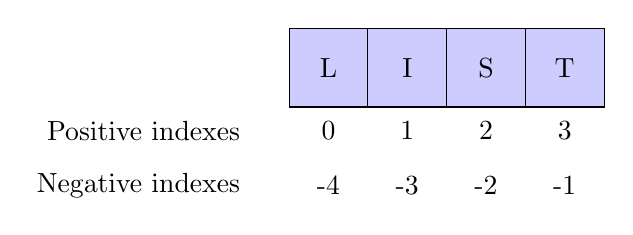
\begin{tikzpicture}
        \filldraw[step=1.0,black, thin, fill=blue!20] (0., 0. ) grid (4, 1) rectangle(0, 0);
        \draw (0.5, 0.5 ) node {L};
        \draw (1.5, 0.5 ) node {I};
        \draw (2.5, 0.5 ) node {S};
        \draw (3.5, 0.5 ) node {T};
        
        \def\wpos{-0.3}
        \def\wneg{-1}
        \def\lab{-0.5}

        \draw (0.5, \wpos ) node {0};
        \draw (1.5, \wpos ) node {1};
        \draw (2.5, \wpos ) node {2};
        \draw (3.5, \wpos ) node {3};
        \draw (\lab, \wpos ) node [anchor=east, align=right]{Positive indexes};
        
        \draw (0.5, \wneg ) node {-4};
        \draw (1.5, \wneg ) node {-3};
        \draw (2.5, \wneg ) node {-2};
        \draw (3.5, \wneg ) node {-1};
        \draw (\lab, \wneg ) node [anchor=east, align=right]{Negative indexes};
    \end{tikzpicture}
\end{document}
